% !TEX root = Projektdokumentation.tex
% \renewcommand\thesection{\Alph{section}}
\renewcommand\thesubsection{\Alph{subsection}}
\section{Anhang}
\subsection{Schnittstelle: ER-Diagramm}
\label{sec:erd-api}
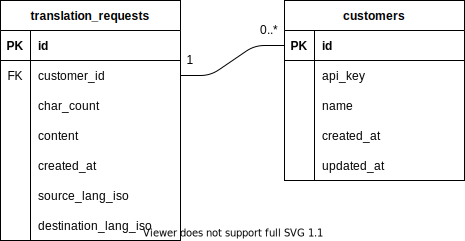
\includegraphics[width=15cm]{./img/ERD-API.pdf}

\subsection{Liste der HTTP-Endpunkte}
\label{sec:table_http_request}
\begin{tabular}{ |l|l|l| }
	\hline
	Methode & URI & Beschreibung \\ 
	\hline
	GET & api/ruok  & Gibt den aktuellen Status der API zurück \\  
	GET & api/translation\_request  & Zeigt alle gespeicherte Datensätze \\  
	POST & api/translation\_request & Schreibt einen Datensatz \\
	GET & api/translation\_request/\{ id \}  & Zeigt einen Datensatz \\  
	PUT & api/translation\_request/\{ id \} & Ändert einen Datensatz \\
	DELETE & api/translation\_request/\{ id \} & Löscht einen Datensatz \\
	\hline
\end{tabular}

\subsection{Tabelle 'translation\_requests'}
\label{sec:table_tranlation_request}
\begin{center}
\begin{tabular}{ |l|l|l|l|l|l|l|l| }
    \hline
    ID & content & source & destination & count & customer\_id  & status & created\_at\\ 
    \hline
    \dots & \dots & \dots & \dots & \dots & \dots & \dots & \dots\\  
    186 & Tisch & DE & EN & 5 & 1 & 200 & 2021-04-29 12:44:48 \\  
    187 & Straße & DE & EN & 7 & 1 & 200 & 2021-04-29 12:45:38 \\  
    188 & Maske & DE & EN & 5 & 2 & 200 & 2021-04-29 12:46:30 \\  
    189 & Uhr & DE & EN & 3 & 1 & 200 & 2021-04-29 12:55:16 \\  
    \dots & \dots & \dots & \dots & \dots & \dots & \dots & \dots\\  
    \hline
\end{tabular}
\end{center}

\subsection{Tabelle 'customers'}
\label{sec:table_customers}

\begin{center}
\begin{tabular}{ |l|l|l|l|l| }
    \hline
    ID & api\_key & name & created\_at & updated\_at \\ 
    \hline
    1 & d6c117cfa61375\dots & langer@[\dots].de & 2021-04-29 12:47:56 & 2021-04-29 12:47:56\\  
    2 & b6f8d434a847fb\dots & birnthaler@[\dots].de & 2021-04-29 12:47:56 & 2021-04-29 12:47:56\\  
    \dots & \dots & \dots & \dots & \dots\\  
    \hline
\end{tabular}
\end{center}

\subsection{Zusatzsoftware: ER-Diagramm}
\label{sec:erd-csharp}
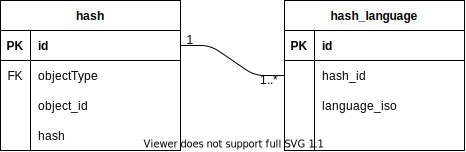
\includegraphics[width=15cm]{./img/ERD-Cscharp.pdf}


\newpage
\subsection{Migration 'translation\_request'}
\label{sec:migration_translation_request}
\begin{lstlisting}[language=php]
<?php

use Illuminate\Database\Migrations\Migration;
use Illuminate\Database\Schema\Blueprint;
use Illuminate\Support\Facades\Schema;

class CreateTranslationRequestsTable extends Migration
{
	// 
	// Run the migrations.
	// @return void
	// 
	public function up()
	{
		Schema::create('translation_requests', function (Blueprint $table) {
			$table->id();

			$table->longText('content');

			$table->string('source_language_iso', 2);
			$table->string('destination_language_iso', 2);

			$table->bigInteger('char_count');
			$table->integer('status');
			$table->foreignId('customer_id')->constrained('customers');

			$table->timestamps();
		});
	}

	// 
	// Reverse the migrations.
	// @return void
	// 
	public function down()
	{
		Schema::dropIfExists('translation_requests');
	}
}
\end{lstlisting}

\newpage
\subsection{Auslesen der Metriken}
\label{sec:sql_data}
\begin{lstlisting}[language=sql]
SELECT  c.name as "Kunde", SUM(char_count) as "Anzahl der Zeichen"
FROM translation_requests as r
JOIN customers c ON r.customer_id = c.id
WHERE r.created_at 
BETWEEN "2021-05-01 00:00:00" AND "2021-05-31 23:59:59"
GROUP BY c.name
\end{lstlisting}

Ausgabe 

\begin{tabular}{|l|r|}
    \hline
    Kunde & Anzahl der Zeichen\\
    \hline
    langer@ris-development.de & 256187\\
    birnthaler@ris-development.de & 65536\\
    \hline
\end{tabular}

\subsection{Model 'TranslationRequest'}
\label{sec:model_translation_request}
\begin{lstlisting}[language=php]
<?php
namespace App\Models;

use Illuminate\Database\Eloquent\Factories\HasFactory;
use Illuminate\Database\Eloquent\Model;

class TranslationRequest extends Model{
    use HasFactory;
    protected $fillable = [
        'content',
        'source_language_iso',
        'destination_language_iso',
        'char_count',
        'status',
        'customer_id',
    ];

    protected $attributes = [
        'char_count' => 0,
        'status' => 1,
    ];
    
    public function setContentAttribute($value){
        $this->attributes['content'] = $value;
        $this->attributes['char_count'] = strlen($value);
    }
}
\end{lstlisting}

\newpage
\subsection{Controller 'TranslationRequest'}
\label{sec:controller_translation_request}
\begin{lstlisting}[language=php]

class TranslationRequestController extends Controller{

    public function store(Request $request){

        $data = $request->validate([
            'content' => "required|min:1",
            'source_language_iso' => "required|size:2",
            'destination_language_iso' => "required|size:2",
            'api_key' => "exists:".Customer::class.",api_key"
        ]);

        $customer = Customer::where('api_key', $data['api_key'])->firstOrFail();

        $data['customer_id'] = $customer->id;
        $translationRequest = TranslationRequest::create($data);
        
        $service = new DeeplService;
        $response = json_decode($service->translate($translationRequest));
        
        //sent request
        $translationRequest->status = 200;
        $translationRequest->save();
        
        return $response->translations[0]->text;
    }
}
\end{lstlisting}

\newpage
\subsection{Service 'DeeplService'}
\label{sec:deeplservice}
\begin{lstlisting}[language=php]
class DeeplService {

    public function translate(TranslationRequest $request){
        $token = config('services.deepl.token');
        $apiUrl = config('services.deepl.api_url');
        
        $response = Http::asForm()->withHeaders([
            'user-agent' => 'BilangApp',
        ])->post($apiUrl, [
            'auth_key' => $token, 
            'text' => $request->content, 
            'target_lang' => $request->destination_language_iso, 
            'source_lang' => $request->source_language_iso, 
            "tag_handling" => "xml"
        ]);
        
        return $response->body();
    }
}
\end{lstlisting}

\subsection{JTL-Ameise GUI: Export}
\label{sec:ameise}
\includegraphics[width=15cm]{./img/AmeiseExport.png}

\newpage
\subsection{Konfigurationsdatei}
\label{sec:config}
\begin{lstlisting}[language=xml]
<?xml version="1.0" encoding="utf-8"?>
<configuration>
    <appSettings>
        <!-- connection to wawi db -->
        <add key="db_server" value="192.168.107.11\DEVWAWI" />
        <add key="db_mandant" value="Mandant_19" />
        <add key="db_pass" value="sa04jT14" />
        <add key="db_user" value="sa" />
        <add key="db_port" value="57981" />

        <!-- Ameisendaten -->
        <add key="jtlAmeisePath" value="C:\Programme\JTL-Software\JTL-wawi-ameise.exe" />
    </appSettings>

    <appLanguages>
        <!-- add key="BG" value="" -->
        <!-- add key="CS" value="" -->
        <!-- add key="DA" value="" -->
        <!-- add key="DE" value="" -->
        <!-- add key="EL" value="" -->
        <add key="EN" value="" />
        <!-- add key="ES" value="" -->
        <!-- add key="ET" value="" -->
        <!-- add key="FI" value="" -->
        <!-- add key="FR" value="" -->
        <!-- add key="HU" value="" -->
        <!-- add key="IT" value="" -->
        <!-- add key="JA" value="" -->
        <!-- add key="LT" value="" -->
        <!-- add key="LV" value="" -->
        <!-- add key="NL" value="" -->
        <!-- add key="PL" value="" -->
        <!-- add key="PT" value="" -->
        <!-- add key="RO" value="" -->
        <!-- add key="RU" value="" -->
        <!-- add key="SK" value="" -->
        <!-- add key="SL" value="" -->
        <!-- add key="SV" value="" -->
        <!-- add key="ZH" value="" -->
    </appLanguages>
</configuration>
\end{lstlisting}


\newpage
\subsection{SqlHelper}
\label{sec:sql_helper}
\begin{lstlisting}[language=php]
using System;
using System.Configuration;
using System.Data.SqlClient;

namespace Bilang.Classes {
    public class SqlHelper {
        public String DbServer { get; set; }
        public String Db { get; set; }
        public String DbUser { get; set; }
        public String DbPass { get; set; }
        public int DbPort { get; set; }
        private String connectionString =>
            "user id=" + DbUser + ";" +
            "password=" + DbPass +
            ";server=" + DbServer+ ((DbPort > 0) ? $",{DbPort}" : "") +
            ";Trusted_Connection=no;Connect Timeout=10;" +
            "Pooling=false;" +
            "database=" + Db + "; " +
            "connection timeout=30";

        public SqlHelper() {
            var config = ConfigurationManager.OpenExeConfiguration(ConfigurationUserLevel.None);
            DbServer = config.AppSettings.Settings["db_server"].Value.Trim();
            Db = config.AppSettings.Settings["db_mandant"].Value.Trim();
            DbUser = config.AppSettings.Settings["db_user"].Value.Trim();
            DbPass = config.AppSettings.Settings["db_pass"].Value.Trim();
            DbPort = int.Parse(config.AppSettings.Settings["db_port"].Value.Trim());
        }
        public void execute(String query) {
            using SqlConnection connection = new SqlConnection(connectionString);
            
            connection.Open();

            SqlCommand execute = new SqlCommand(query, connection);
            execute.ExecuteNonQuery();
            Console.WriteLine("Inserting Data Successfully");

            connection.Close();
        }
    }
}
\end{lstlisting}

\subsection{Tabelle 'hash'}
\label{sec:table_hash}
\begin{tabular}{ |l|l|l|l|l| }
	\hline
	ID & object\_type & object\_id & hash \\ 
	\hline
	\dots & \dots & \dots & \dots\\  
	255 & kArtikel & 45621 & e3b0c44298fc1c149\dots\\  
	256 & kArtikel & 45621 & 9f86d081884c7d659\dots\\  
	257 & kKategorie & 19017 & 34ca495991b7852b8\dots\\  
	\dots & \dots & \dots & \dots\\  
	\hline
\end{tabular}

\subsection{Tabelle 'hash\_language'}
\label{sec:table_hash_language}
\begin{tabular}{ |l|l|l|l|l| }
	\hline
	ID & hash\_id & language\_iso \\ 
	\hline
	\dots & \dots & \dots \\  
	419 & 255 & EN\\  
	420 & 255 & NL\\  
	410 & 256 & EN\\  
	\dots & \dots & \dots \\  
	\hline
\end{tabular}

\newpage
\subsection{ApiHelper}
\label{sec:api_helper}
\begin{lstlisting}[language=php]
public static string PostRequest(string url, string payload) {

    HttpWebRequest request = (HttpWebRequest)WebRequest.Create(url);
    request.Method = "POST";
    request.ContentType = "application/json";

    using(var streamWriter = new StreamWriter(request.GetRequestStream())) {
        streamWriter.Write(payload);
    }

    HttpWebResponse response = null;
    string responseStr = "";

    try {
        response = (HttpWebResponse)request.GetResponse();
        responseStr = ReadAllFromResponse(response);
    }
    catch(WebException e) {
        Console.Write("---\tError in request:\n" + e + "\n---");
    }

    using(var streamReader = new StreamReader(response.GetResponseStream())) {
        var result = streamReader.ReadToEnd();
    }

    return responseStr;
}
\end{lstlisting}

\subsection{Weichstelle der API für Tests}
\label{sec:testing_api}
\begin{lstlisting}[language=php]
if($data['api_key'] == "9876543210"){
    return $data['destination_language_iso']."(".$data['content'].")";
}
\end{lstlisting}